\section{Allgemeines}

\subsection{Definition: Embedded System}
\begin{itemize}
	
	\item \underline{Rechner} ist in einem \underline{technischen} Kontext integriert/eingebettet
	
	\item Wird eingesetzt um: \underline{Steuerung}, \underline{Regelung}, \underline{Überwachung} eines technischen Prozesses umzusetzen

	\item nur für eine \underline{spezifische} Aufgabe entwickelt (evtl. \underline{Echtzeitanforderung})
	
	\item Aspekte:
	\begin{itemize}
		\item Resourcenverbrauch
		\item Kombination von Hard und Software
		\item Kosteneffizienz bei der Herstellung
	\end{itemize}
	
\end{itemize}

\subsection{Interaktion mit der Umwelt}
\begin{figure}[h!]
	\begin{center}
		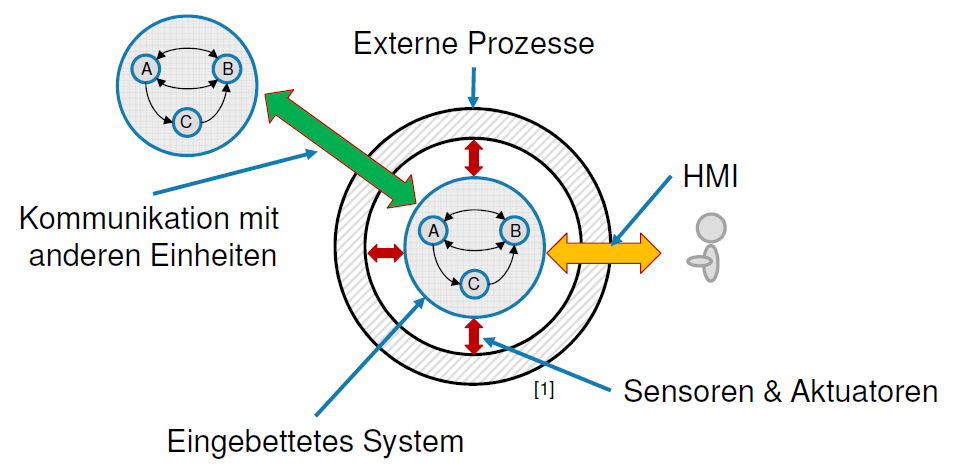
\includegraphics[width=.5\linewidth]{pics/interaktion}
		\caption{Eingebettetes System: Integration und Interaktion mit der Umwelt}
	\end{center}
\end{figure}

\subsection{Definition: Prozess}
Gesamtheit von \underline{aufeinander einwirkenden Vorgängen} in einem System, 
durch die Materie, Energie oder Information umgeformt, transportiert oder gespeichert wird

\begin{itemize}
	\item Technischer Prozess \\
	Prozess in dem die Zustandsgrößen durch technische Hilfsmittel
	festgestellt und beeinflusst werden (Sensoren/Aktuatoren)
	
	\item Rechenprozess
	\begin{itemize}
		\item Umformen, Transportieren, Speichern von Information
		\item Berechnen von Ausgabewerten aus Eingabewerten
		\item Beschrieben durch ein Programm
	\end{itemize}
	
	\item Kognitiver Prozess
	
\end{itemize}

\begin{figure}[h!]
	\begin{center}
		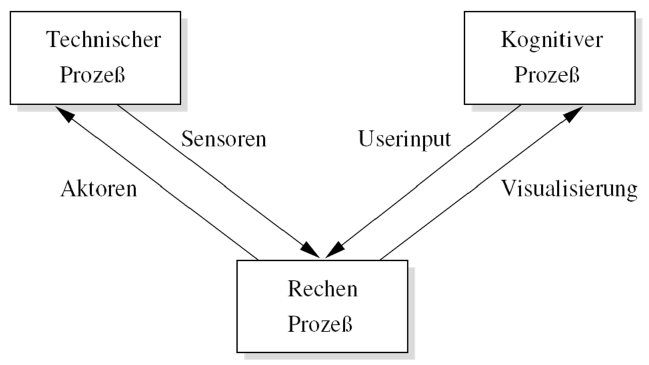
\includegraphics[width=.5\linewidth]{pics/prozesse}
		\caption{Zusammenwirken der Prozesse}
	\end{center}
\end{figure}

\subsection{Steuerung vs Regelung}
Bei Regelung werden Sensorwerte verwendet für Steuerung.

\subsection{Klassifizierung: Technischer Prozess}
\begin{itemize}

	\item Fließprozess (kontinuierlich/dynamisch) $\Rightarrow$ Regler
	
	\item Folgeprozess (diskrete Informationselemente) $\Rightarrow$ State Machine
	
	\item Stückprozess (Transport, Laden, Fertigen) $\Rightarrow$ Datenbank

\end{itemize}